\nxsection{Le r\^ole ''Magasinier''}\label{sec:utilisateurs-lemagasinier}
\index{magasinier}
\index{LeMagasinier}

La figure~\ref{fig:yeren-fenetre-magasinier} illustre
la fen\^etre d'acceuil d'un utilisateur avec le
\role \magasinier, apr\`es qu'il se soit enregistr\'e
dans \yeren.\\

\begin{figure}[!htbp]
\centering
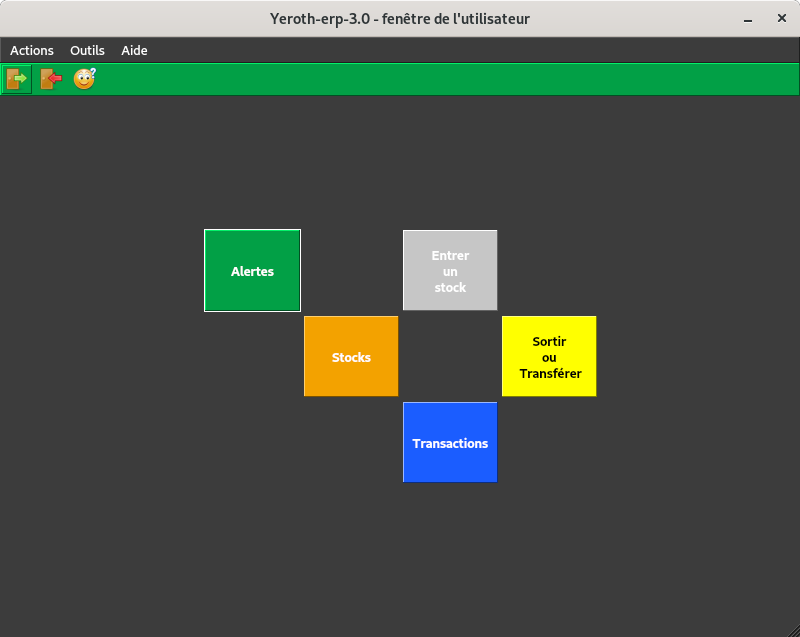
\includegraphics[scale=0.63]{images/yeren-fenetre-magasinier.png}
\caption{La fen\^etre d'acceuil d'un magasinier.}
\label{fig:yeren-fenetre-magasinier}
\end{figure}

Un utilisateur de \yeren avec le \role "\magasinier" assume les
t\^aches suivantes:
\begin{enumerate}[1)]
	\item lister des stocks
	\item modifier un stock
	\item rechercher des articles / stocks
	\item rechercher des transactions 
		(sorties de stocks ou transferts de stocks)
	\item sortir des articles / stocks
	\item supprimer un stock
	\item transf\'erer un stock
	\item visualiser des transactions
	(sorties de stocks ou transferts de stocks).\\
\end{enumerate}

\magasinier n'a pas acc\`es aux fonctions
\bouton{Administration}, \bouton{Ventes},
\bouton{Rapports}, et \bouton{Vendre}.

On remarque sur la Figure~\ref{fig:yeren-fenetre-magasinier}
que les boutons \bouton{Administration}, \bouton{Ventes},
\bouton{Rapports}, et \bouton{Vendre} sont d\'esactiv\'es.